\documentclass[11pt,a4paper]{article}

\usepackage[utf8]{inputenc}%
\usepackage[margin=1in]{geometry}%
\usepackage{manyfoot}%
\usepackage{graphicx}%
\usepackage{multirow}%
\usepackage{booktabs}%
\usepackage{amsmath,amssymb,amsfonts}%
\newcommand{\ket}[1]{\left|#1\right\rangle}
\usepackage{xcolor}%
\usepackage{tikz}%
\usepackage{pgfplots}%
\pgfplotsset{compat=1.18}%
\usepackage{caption}%
\usepackage{placeins}%
\usepackage[numbers,sort&compress]{natbib}%
\bibliographystyle{unsrt}%

\raggedbottom

\title{\textbf{Hybrid Quantum-Classical Framework for Multi-Label Bengali Emotion Classification}}

\author{%
Tathagata Mitra, Biswanath Ranjit\\[2pt]
Pritam Pal, Dipankar Das\\[4pt]
\small Department of Physics, Jadavpur University, Kolkata, West Bengal, India\\[2pt]
\small Department of Computer Science, Jadavpur University, Kolkata, West Bengal, India}

\date{}

\begin{document}

\maketitle

\begin{abstract}
Multi-label emotion classification of code-mixed and low-resource languages such as Bengali remains a challenging task because of limited labelled corpora, severe class imbalance, and the need to recognise multiple co-occurring emotions per comment. This paper investigates hybrid quantum-classical models that combine pretrained transformer representations with trainable variational quantum circuits (VQCs) for six-way multi-label emotion classification on the EmoNoBa dataset. We design two custom four-qubit VQC architectures---a cross-coupling entangling scheme (Custom 1) and a re-uploading encoding scheme with a rotating ansatz (Custom 2)---and evaluate them with two Bengali encoders (IndicBERTv2 and BanglaBERT) across 2, 4, and 8-qubit registers. In addition to the per-label macro, micro, and weighted F1-scores, we report the Exact Match Ratio (EMR) and an instance-level partial-match F1-score. The quantum variants substantially improve the weaker BanglaBERT baseline, raising its macro F1-score from 0.2101 to 0.4850 and its EMR from 0.0000 to 0.4630, while the best overall macro F1-score of 0.5165 and the highest EMR of 0.4577 are achieved with IndicBERTv2 and Custom 2 at eight qubits. Our results indicate that the benefit of additional qubits depends critically on the compatibility of the encoding, entanglement pattern, and classical representation.
\end{abstract}

\noindent\textbf{Keywords:} hybrid quantum-classical machine learning, variational quantum circuits, multi-label emotion classification, Bengali natural language processing, low-resource languages, exact match ratio

\vspace{1em}

\section{Introduction}\label{sec:intro}
Multi-label emotion classification is an important natural language processing (NLP) task with applications in sentiment-aware dialogue systems, social-media analysis, public-opinion monitoring, and human--computer interaction. Unlike binary sentiment analysis, which assigns a single polarity, multi-label emotion recognition requires a model to predict a set of emotions for each input, since closely related emotions frequently co-occur. The problem becomes substantially more difficult for low-resource languages such as Bengali, because labelled corpora, language-specific pretrained models, balanced emotion datasets, and standardized benchmarks are comparatively limited \cite{bhattacharjee2022banglabert,islam2022emonoba}. Minority emotion classes are easily suppressed by dominant labels, and the informal, noisy style of social-media text compounds the difficulty.

In parallel, near-term quantum machine learning (QML) has emerged as a promising paradigm in which parameterized quantum circuits (PQCs) map classical feature vectors into high-dimensional quantum Hilbert spaces \cite{huzzat2026primer}. Variational quantum circuits---PQCs with trainable rotation parameters updated by gradient descent---have been applied to supervised learning \cite{schuld2020circuit}, and the data re-uploading paradigm interleaves classical feature encoding layers $U(x)$ with trainable unitaries $U(\theta)$ to increase the expressivity of low-qubit circuits \cite{perez2020data}. Recent analyses of parameterized circuit expressibility and entanglement \cite{sim2019expressibility} and of hybrid quantum-classical training dynamics \cite{arthur2022hybrid} provide a theoretical basis for designing trainable quantum feature extractors. These developments motivate the question of whether a variational quantum circuit, inserted as a trainable bottleneck inside a classical transformer architecture, can improve multi-label emotion classification for Bengali.

In this paper, we present a hybrid quantum-classical framework that combines a pretrained Bengali transformer encoder with a trainable variational quantum circuit for multi-label emotion classification on the EmoNoBa dataset \cite{islam2022emonoba}. The contributions of this paper are as follows:
\begin{itemize}
    \item We develop a hybrid quantum-classical framework that couples a pretrained Bengali transformer encoder (IndicBERTv2 \cite{doddapaneni2023towards} or BanglaBERT \cite{bhattacharjee2022banglabert}) with a trainable variational quantum circuit for six-way multi-label emotion classification, and a classical baseline without a quantum branch.
    \item We design and compare two custom four-qubit VQC architectures---a cross-coupling entangling scheme (Custom 1) and a re-uploading encoding scheme with a rotating ansatz (Custom 2)---under an identical outer framework, and evaluate both across 2, 4, and 8-qubit registers.
    \item We evaluate all configurations with a unified protocol covering per-label macro, micro, and weighted F1-scores, the Hamming loss, the Exact Match Ratio (EMR), and an instance-level partial-match F1-score, and analyse how encoding, entanglement, and circuit depth interact with the quality of the classical representation.
\end{itemize}

The remainder of this paper is organized as follows. Section~\ref{sec:related} reviews related work on low-resource Bengali NLP and on quantum machine learning. Section~\ref{sec:dataset} describes the EmoNoBa dataset and its label distribution. Section~\ref{sec:method} presents the task definition, the overall architecture, the two VQC designs, the training setup, and the evaluation metrics. Section~\ref{sec:experiments} describes the experimental setup and reports the results. Section~\ref{sec:discussion} discusses the findings, Section~\ref{sec:conclusion} concludes the paper, and Section~\ref{sec:limitations} outlines the limitations of the present work.

\section{Related Work}\label{sec:related}
In this section, we discuss related work spanning four areas: Bengali and Indic natural language processing, multi-label emotion and sentiment classification, quantum natural language processing, and variational quantum circuits applied to NLP. Although quantum computing has received growing interest over the last decade, its application to NLP---and especially to low-resource languages such as Bengali---remains comparatively underexplored \cite{varmantchaonala2024quantum}.

\subsection{Bengali and Indic Language Processing}\label{sec:related-bengali}
Bengali is the seventh most widely spoken language in the world, with over 272 million speakers concentrated primarily in India and Bangladesh, yet it remains significantly underrepresented in NLP research compared with high-resource languages such as English \cite{das2010emotion}. The scarcity of annotated corpora, standardized benchmarks, and language-specific pretrained models has historically limited the performance of downstream tasks including sentiment analysis, emotion recognition, and text classification.

Early computational work on Bengali emotion analysis was pioneered by Das and Bandyopadhyay \cite{das2010emotion}, who developed rule-based and lexicon-based methods for identifying emotions in Bengali text. More recently, the release of large-scale pretrained language models has substantially advanced the state of the art. Bhattacharjee et al.\ \cite{bhattacharjee2022banglabert} introduced BanglaBERT, a BERT-based model pretrained on a large corpus of Bangla text, and demonstrated its effectiveness across several low-resource language understanding benchmarks. Doddapaneni et al.\ \cite{doddapaneni2023towards} developed IndicBERTv2 as part of a broader effort to build monolingual corpora, benchmarks, and models for Indic languages, showing that language-specific pretraining consistently outperforms multilingual baselines such as mBERT and XLM-R \cite{devlin2019bert,conneau2020xlmr}. These encoders provide the contextual text representations used in our hybrid framework.

The EmoNoBa dataset, introduced by Islam et al.\ \cite{islam2022emonoba}, is a manually annotated collection of 22,698 noisy Bangla social-media comments labelled with six fine-grained emotion categories based on the Junto Emotion Wheel. It preserves the informal and code-mixed characteristics of online Bengali text and has become a standard benchmark for multi-label emotion classification in this language. The strong class imbalance in the dataset---where \emph{Joy} dominates and \emph{Fear} is severely underrepresented---has motivated the use of class-weighted loss functions and threshold calibration in subsequent studies.

\subsection{Multi-Label Emotion and Sentiment Classification}\label{sec:related-multilabel}
Multi-label classification assigns a set of non-exclusive labels to each input instance, in contrast to multi-class classification, which selects a single category. Tsoumakas and Katakis \cite{tsoumakas2007multi} provided a comprehensive overview of multi-label learning approaches, categorizing them into problem-transformation methods (e.g.\ binary relevance, classifier chains) and algorithm-adaptation methods (e.g.\ multi-label $k$-nearest neighbours, ranking-based losses). Zhang and Zhou \cite{zhang2014review} later surveyed multi-label learning algorithms, formalizing the connections between label correlations, evaluation metrics, and algorithmic design.

In the context of emotion recognition, the multi-label formulation is essential because closely related emotions frequently co-occur in a single utterance---for instance, a comment may simultaneously express both \emph{Joy} and \emph{Love}, or both \emph{Anger} and \emph{Sadness}. Classical approaches to multi-label emotion classification typically employ independent binary classifiers per label (binary relevance) followed by a sigmoid activation and a fixed threshold of 0.5 \cite{bishop2006pattern}. However, fixed thresholds lead to poor performance on imbalanced datasets, and strict evaluation criteria such as the Exact Match Ratio (EMR)---which requires the entire predicted label vector to match the gold vector---amplify this problem. Our framework addresses these issues through per-label positive-weight calibration in the loss function and per-emotion threshold tuning on the validation set.

\subsection{Quantum Natural Language Processing}\label{sec:related-qnlp}
Quantum computing, grounded in quantum-mechanical phenomena such as superposition and entanglement, offers the potential to solve certain computational problems more efficiently than classical computers \cite{huzzat2026primer}. One of the earliest intersections of quantum theory and NLP was the work of Basile and Tamburini \cite{basile2017quantum}, who proposed quantum language models using quantum probability theory and showed that their models outperform classical language models in terms of perplexity scores. Tamburini \cite{tamburini2019quantum} subsequently applied quantum probability theory to word sense disambiguation.

In the area of sentiment and emotion analysis, Liu et al.\ \cite{liu2021quantum} proposed a joint multi-modal multi-task learning framework for sentiment and sarcasm detection using quantum probability, evaluating their model on the MUStARDext \cite{chauhan2020sentiment} and Memotion \cite{sharma2020semeval} datasets and demonstrating state-of-the-art performance. Phukan and Ekbal \cite{phukan2023qemma} proposed QeMMA, a quantum-enhanced multi-modal sentiment analysis framework utilizing variational quantum circuits, and showed improvements on the CMU-MOSEI dataset. Li et al.\ \cite{li2021qtns} explored a quantum-inspired multimodal fusion framework for sentiment analysis, further demonstrating the utility of quantum-inspired methods in affective computing. Zhang et al.\ \cite{zhang2019quantum} developed quantum-inspired interactive networks for conversational sentiment analysis, leveraging quantum probability to model contextual dependencies in dialogue.

Part-of-speech (POS) tagging has also been explored using quantum methods. Di~Sipio et al.\ \cite{disipio2021dawn} investigated quantum natural language processing approaches including quantum long short-term memory (QLSTM) networks. Pandey et al.\ \cite{pandey2022pos} applied unidirectional QLSTM to POS tagging in Mizo, a low-resource Indian language, while Pandey and Pakray \cite{pandey2023bqlstm} used bidirectional QLSTM for POS tagging on code-mixed texts. Pal and Das \cite{pal2025quantum} developed a hybrid classical-quantum framework for sentiment classification and claim check-worthiness identification in Bengali using QLSTM, providing one of the few studies that apply quantum methods to Bengali NLP.

Quantum frameworks have been explored in several other NLP tasks as well, including text classification \cite{xu2024quantum,shi2023quantum}, claim identification \cite{pal2025quantum}, and metaphor detection \cite{qiao2024quantum}. Xu et al.\ \cite{xu2024quantum} used quantum recurrent neural networks (quantum RNNs) for text classification and evaluated their models on the Rotten Tomatoes dataset. Shi et al.\ \cite{shi2023quantum} developed quantum-inspired convolutional neural network-based models and evaluated them on popular benchmark datasets such as SST, SUBJ, and MPQA. Yan et al.\ \cite{yan2024quantum} proposed a quantum-inspired language model with Lindblad master equations and interference measurement for sentiment analysis. Qiao et al.\ \cite{qiao2024quantum} introduced a quantum-inspired matching network with linguistic theories for metaphor detection.

Coecke et al.\ \cite{coecke2020foundations} proposed the DisCoCat framework, a categorical approach to quantum NLP that preserves the linguistic meaning and compositional structure of a text and converts them into quantum circuits. The applications of the DisCoCat framework have been demonstrated in several studies. Ruskanda et al.\ \cite{ruskanda2022quantum,ruskanda2023simple} performed sentiment analysis using the DisCoCat framework with the \texttt{lambeq} toolkit \cite{kartsaklis2021lambeq}, an open-source Python library for quantum natural language processing. Ganguly et al.\ \cite{ganguly2022quantum} also applied the DisCoCat framework for sentiment classification. These compositional approaches contrast with the feature-extraction paradigm used in the present work, where a pretrained transformer provides dense embeddings that are subsequently processed by a variational quantum circuit.

There are several comprehensive survey papers that discuss quantum NLP and its applications. Wu et al.\ \cite{wu2021quantum} categorized different quantum algorithms and NLP tasks, concluding that quantum NLP models produce better or equivalent results to classical NLP models. Guarasci et al.\ \cite{guarasci2022quantum} reviewed the challenges and opportunities in quantum NLP. Varmantchaonala et al.\ \cite{varmantchaonala2024quantum} provided a comprehensive survey of quantum NLP, while Widdows et al.\ \cite{widdows2024quantum} discussed the state of the art and future directions.

\subsection{Variational Quantum Circuits for Machine Learning}\label{sec:related-vqc}
Variational quantum circuits (VQCs), also called parameterized quantum circuits (PQCs), are a class of quantum circuits with trainable rotation parameters that are updated by classical gradient-based optimization \cite{benedetti2019parameterized,mcclean2016theory}. They form the core computational element in near-term quantum machine learning and are particularly suited to hybrid quantum-classical architectures operating on noisy intermediate-scale quantum (NISQ) devices.

Schuld et al.\ \cite{schuld2020circuit} established circuit-centric quantum classifiers and demonstrated that parameterized circuits can be trained for supervised classification tasks. Arthur and Date \cite{arthur2022hybrid} investigated hybrid quantum-classical neural networks and analysed the training dynamics of variational circuits when coupled with classical layers. P\'erez-Salinas et al.\ \cite{perez2020data} introduced the data re-uploading paradigm, in which classical feature-encoding layers $U(x)$ are interleaved with trainable unitary transformations $U(\theta)$ across $L$ layers:
\begin{equation}
U(\theta, x) = \prod_{l=1}^{L} U(\theta_l)\, U(x) .
\label{eq:reupload}
\end{equation}
Repeatedly injecting the input allows constrained circuits to represent more complex decision functions than a single encoding layer, effectively making a single qubit a universal classifier.

The design of the variational ansatz critically affects the expressivity and trainability of the circuit. Sim et al.\ \cite{sim2019expressibility} analysed the expressibility and entangling capability of parameterized circuits and showed that the choice of gate family and entanglement structure directly affects the representational power of the ansatz. Qin \cite{qin2023review} reviewed ansatz-design techniques for variational quantum algorithms, summarizing trade-offs between circuit depth, trainability, and hardware efficiency. McClean et al.\ \cite{mcclean2018barren} identified the barren-plateau phenomenon, showing that gradients of randomly initialized deep circuits can vanish exponentially with the number of qubits, which motivates the use of shallow, structured ansatze. Schuld et al.\ \cite{schuld2021quantum} analysed the effect of data encoding on the expressive power of variational quantum machine-learning models, showing that the choice of encoding strategy is as important as the variational ansatz itself.

Beyond supervised classification, variational circuits have been applied to a broad range of machine-learning tasks. Chen et al.\ \cite{chen2020vqc} applied variational quantum circuits to deep reinforcement learning, demonstrating that quantum agents can match or exceed classical agents in several benchmark environments. Kandala et al.\ \cite{kandala2017hardware} demonstrated hardware-efficient variational quantum eigensolvers for small molecules and quantum magnets, establishing the practical viability of variational ansatze on real quantum hardware. Huzzat et al.\ \cite{huzzat2026primer} provided a primer on quantum neural network models for text classification, covering the end-to-end design from concept to deployment.

Building on these foundations, the present work combines a pretrained Bengali transformer feature extractor with trainable variational quantum circuits, employing both a cross-coupling entangling scheme and a data-re-uploading scheme with per-label decision-threshold calibration, targeting class imbalance and joint subset-prediction accuracy in multi-label Bengali emotion classification.

\section{Dataset}\label{sec:dataset}
This study uses the EmoNoBa dataset, a manually annotated collection of 22,698 public Bangla comments gathered from social media platforms \cite{islam2022emonoba}. The comments span 12 domains, including personal matters, politics, and health, and are labelled with six fine-grained emotion categories based on the Junto Emotion Wheel. The dataset preserves the informal and noisy characteristics of online Bangla text, making it suitable for evaluating emotion-classification models under realistic conditions.

The dataset is split into training, validation, and test partitions of 18,420, 2,047, and 2,272 comments, respectively. Table~\ref{tab:labels} reports the per-emotion label counts in the training partition. The distribution is strongly imbalanced: \emph{Joy} (8,314) dominates, whereas \emph{Surprise} (848) and especially \emph{Fear} (279) are severely underrepresented. As discussed in Section~\ref{sec:training}, this imbalance motivates the use of per-label positive weights in the binary cross-entropy loss to prevent the minority emotion classes from being suppressed.

\begin{table}[htbp]
\centering
\caption{Distribution of emotion labels in the training partition of the EmoNoBa dataset.}
\label{tab:labels}
\begin{tabular}{lcc}
\toprule
\textbf{Emotion} & \textbf{Count} & \textbf{Percentage} \\
\midrule
Joy      & 8,314 & 45.14 \\
Sadness  & 4,569 & 24.80 \\
Love     & 3,786 & 20.55 \\
Anger    & 3,542 & 19.23 \\
Surprise &   848 &  4.60 \\
Fear     &   279 &  1.51 \\
\midrule
Total    & 18,420 & 100.00 \\
\bottomrule
\end{tabular}
\end{table}

\section{Methodology}\label{sec:method}

\subsection{Task Definition}\label{sec:task}
Given a Bengali comment $x$ consisting of a sequence of tokens, the objective is to predict a binary label vector $y \in \{0, 1\}^{K}$ over $K = 6$ emotion categories---\emph{Love, Joy, Surprise, Anger, Sadness, Fear}---where $y_k = 1$ indicates that emotion $k$ is expressed in the comment and multiple emotions may co-occur. Following the convention of multi-label classification, the model produces an independent logit $z_k$ for each emotion, which is converted to a probability via the sigmoid function $\sigma(z_k) = 1/(1 + e^{-z_k})$ and thresholded at $0.5$ to obtain the predicted label $\hat{y}_k$. The goal is to maximise joint subset-prediction accuracy, measured by the Exact Match Ratio, while retaining competitive per-label performance.

\subsection{Framework Description}\label{sec:framework}
Figure~\ref{fig:pipeline} provides an overview of the proposed hybrid classical-quantum framework. For both the classical baseline and the quantum variants, each comment is first tokenized with a maximum sequence length of 128 and passed through a pretrained Bengali transformer encoder, either IndicBERTv2 or BanglaBERT, from which the 768-dimensional [CLS] representation is extracted. A trainable linear layer projects this representation to a 128-dimensional feature vector, which is then squashed by a $\tanh$ activation.

In the quantum variant, the compressed features are further projected by a linear layer into a low-dimensional vector matching the qubit register (e.g.\ four features for a four-qubit circuit) and fed into the variational quantum circuit described in Section~\ref{sec:vqc}. The expectation values produced by the circuit are mapped back through a post-quantum linear layer to the 128-dimensional working space, followed by a ReLU activation. In the classical baseline, the quantum block is removed and the 128-dimensional features are passed directly to the classifier. In both cases, a final linear layer maps the representation to the $K = 6$ logits, which are interpreted with sigmoid outputs for multi-label prediction.

\begin{figure}[htbp]
\centering
\resizebox{\textwidth}{!}{%
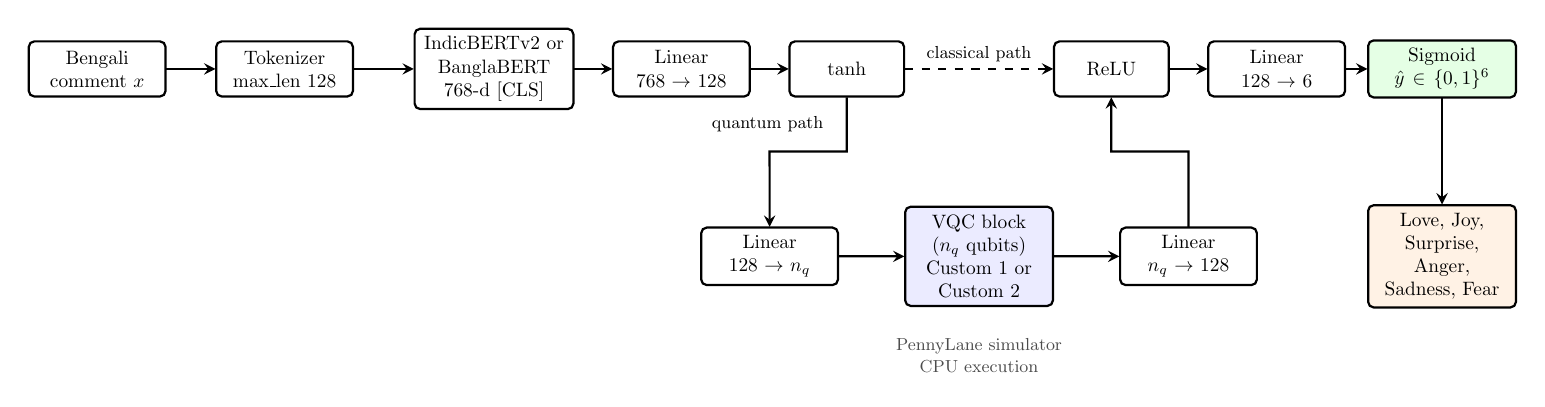
\begin{tikzpicture}[
    box/.style={draw, rounded corners=2pt, thick, fill=white, align=center, inner sep=4pt},
    arr/.style={-stealth, thick},
    scale=0.7,
    every node/.style={transform shape}
]
    \node[box, minimum height=1.0cm, text width=2.2cm] (in) at (0,0) {Bengali\\comment $x$};
    \node[box, minimum height=1.0cm, text width=2.2cm] (tok) at (3.4,0) {Tokenizer\\max\_len 128};
    \node[box, minimum height=1.0cm, text width=2.6cm] (enc) at (7.2,0) {IndicBERTv2 or\\BanglaBERT\\768-d [CLS]};
    \node[box, minimum height=1.0cm, text width=2.2cm] (lin) at (10.6,0) {Linear\\768 $\rightarrow$ 128};
    \node[box, minimum height=1.0cm, text width=1.8cm] (tanh) at (13.6,0) {$\tanh$};
    \node[box, minimum height=1.0cm, text width=1.8cm] (relu) at (18.4,0) {ReLU};
    \node[box, minimum height=1.0cm, text width=2.2cm] (clf) at (21.4,0) {Linear\\128 $\rightarrow$ 6};
    \node[box, minimum height=1.0cm, text width=2.4cm, fill=green!10] (out) at (24.4,0) {Sigmoid\\$\hat{y} \in \{0,1\}^6$};

    \node[box, minimum height=1.0cm, text width=2.2cm] (preq) at (12.2,-3.4) {Linear\\128 $\rightarrow$ $n_q$};
    \node[box, minimum height=1.8cm, text width=2.4cm, fill=blue!8] (vqc) at (16.0,-3.4) {VQC block\\($n_q$ qubits)\\Custom 1 or Custom 2};
    \node[box, minimum height=1.0cm, text width=2.2cm] (postq) at (19.8,-3.4) {Linear\\$n_q$ $\rightarrow$ 128};

    \draw[arr] (in) -- (tok);
    \draw[arr] (tok) -- (enc);
    \draw[arr] (enc) -- (lin);
    \draw[arr] (lin) -- (tanh);

    \draw[arr, dashed] (tanh) -- node[above, font=\small] {classical path} (relu);
    \draw[arr] (relu) -- (clf);
    \draw[arr] (clf) -- (out);

    \draw[arr] (tanh.south) -- (13.6,-1.5) -- (12.2,-1.5) -- (preq.north);
    \node[font=\small, anchor=east] at (13.3,-1.0) {quantum path};
    \draw[arr] (preq) -- (vqc);
    \draw[arr] (vqc) -- (postq);

    \draw[arr] (postq.north) -- (19.8,-1.5) -- (18.4,-1.5) -- (relu.south);

    \node[box, minimum height=1.0cm, text width=2.4cm, fill=orange!10] (lab) at (24.4,-3.4) {Love, Joy,\\Surprise, Anger,\\Sadness, Fear};
    \draw[arr] (out.south) -- (lab.north);

    \node[font=\small, align=center, text=black!70] at (16.0,-5.2) {PennyLane simulator\\CPU execution};
\end{tikzpicture}%
}
\caption{End-to-end framework of the hybrid classical-quantum model for multi-label Bengali emotion classification. The dashed classical path corresponds to traditional pipelines, where the compressed text representation is fed directly to the classifier without any quantum component; it is shown for reference and is not a branch in our model. The solid quantum path inserts the variational quantum circuit between the compressed text representation and the post-quantum fusion layer, replacing the direct classical connection in the proposed framework.}
\label{fig:pipeline}
\end{figure}

\subsection{VQC Designs}\label{sec:vqc}
Following the transformer encoding, the 768-dimensional CLS embedding is projected by a trainable linear layer to a low-dimensional feature vector. Depending on the variant, the vector is squashed by $\tanh$ and fed directly into a four-qubit variational quantum circuit (VQC); the circuit outputs are mapped back through a post-quantum linear layer and a ReLU activation before the final classifier. Three VQCs are investigated: a reference strongly-entangling circuit (SEL), designed by Pritam Pal, and two custom designs---Custom~1, developed by Biswanath Ranjit, and Custom~2, developed by Tathagata Mitra.

\paragraph{SEL reference VQC.}
This circuit acts on $n_q \in \{2, 4, 8\}$ qubits and consumes an $\mathbb{R}^{n_q}$ vector.
\begin{enumerate}
    \item[(i)] \textbf{Encoding.} Each feature is directly injected as a single-axis rotation $R_X(x_i)$ on qubit $i$ (angle embedding).
    \item[(ii)] \textbf{Ansatz.} A single variational layer of PennyLane's \texttt{StronglyEntanglingLayers} is applied, which places a general single-qubit rotation Rot on every qubit and then entangles all qubits with CNOT gates, producing $3 n_q$ trainable parameters. No data re-uploading is performed.
    \item[(iii)] \textbf{Measurement.} The Pauli-$Z$ expectation is measured on every qubit, producing $n_q$ outputs for the post-quantum linear layer.
\end{enumerate}

\begin{figure}[htbp]
\centering
\resizebox{0.72\textwidth}{!}{%
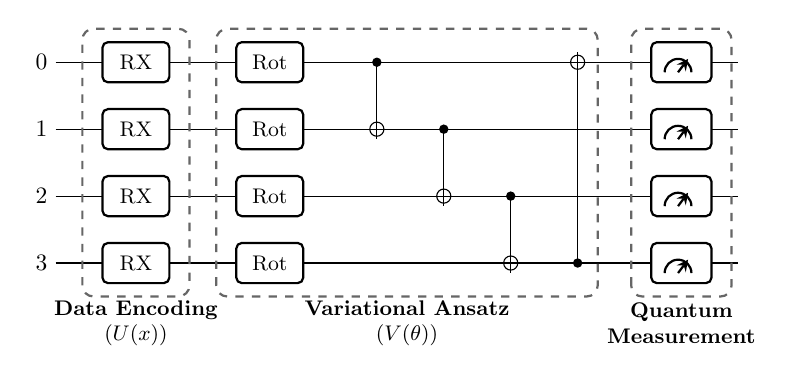
\begin{tikzpicture}[scale=0.85, every node/.style={transform shape}]
    \draw (0,3) node[left] {$0$} -- (10.2,3);
    \draw (0,2) node[left] {$1$} -- (10.2,2);
    \draw (0,1) node[left] {$2$} -- (10.2,1);
    \draw (0,0) node[left] {$3$} -- (10.2,0);

    % --- Data Encoding U(x) ---
    \foreach \y in {0,1,2,3} {
        \draw[fill=white, rounded corners=2pt, thick] (0.7,\y-0.3) rectangle (1.7,\y+0.3) node[midway] {\small RX};
    }
    \draw[dashed, thick, black!60, rounded corners=4pt] (0.4,-0.5) rectangle (2.0,3.5);
    \node[font=\small\bfseries, align=center] at (1.2,-0.9) {Data Encoding\\$(U(x))$};

    % --- Variational Ansatz V(theta) ---
    \foreach \y in {0,1,2,3} {
        \draw[fill=white, rounded corners=2pt, thick] (2.7,\y-0.3) rectangle (3.7,\y+0.3) node[midway] {\small Rot};
    }

    \fill (4.8,3) circle (2pt); \draw (4.8,2) circle (3pt); \draw (4.5,2) -- (5.1,2); \draw (4.8,3) -- (4.8,1.85);
    \fill (5.8,2) circle (2pt); \draw (5.8,1) circle (3pt); \draw (5.5,1) -- (6.1,1); \draw (5.8,2) -- (5.8,0.85);
    \fill (6.8,1) circle (2pt); \draw (6.8,0) circle (3pt); \draw (6.5,0) -- (7.1,0); \draw (6.8,1) -- (6.8,-0.15);
    \fill (7.8,0) circle (2pt); \draw (7.8,3) circle (3pt); \draw (7.5,3) -- (8.1,3); \draw (7.8,0) -- (7.8,3.15);

    \draw[dashed, thick, black!60, rounded corners=4pt] (2.4,-0.5) rectangle (8.1,3.5);
    \node[font=\small\bfseries, align=center] at (5.25,-0.9) {Variational Ansatz\\$(V(\theta))$};

    % --- Quantum Measurement ---
    \foreach \y in {0,1,2,3} {
        \draw[fill=white, rounded corners=2pt, thick] (8.9,\y-0.3) rectangle (9.8,\y+0.3);
        \draw[thick] (9.1,\y-0.15) arc (180:0:0.2);
        \draw[-stealth, thick] (9.3,\y-0.15) -- (9.45,\y+0.05);
    }
    \draw[dashed, thick, black!60, rounded corners=4pt] (8.6,-0.5) rectangle (10.1,3.5);
    \node[font=\small\bfseries, align=center] at (9.35,-0.9) {Quantum\\Measurement};
\end{tikzpicture}%
}
\caption{Four-qubit circuit architecture used for the SEL VQC.}
\label{fig:sel}
\end{figure}

\paragraph{Custom 1 cross-coupling VQC.}
This circuit acts on $n=4$ qubits and consumes an $\mathbb{R}^{4}$ vector.
\begin{enumerate}
    \item[(i)] \textbf{Encoding.} Each feature is directly injected as a single-axis rotation $R_Y(x_i)$ on qubit $i$ (angle embedding).
    \item[(ii)] \textbf{Ansatz.} Two variational layers are used, each consisting of a general Rot applied to every qubit followed by a controlled-NOT entangling stage. The first stage uses a nearest-neighbour ring, with CNOT gates on (0, 1), (1, 2), (2, 3), and (3, 0); the second uses a cross-coupling pattern, with CNOT gates on (0, 2), (1, 3), (2, 1), and (3, 0). The same 12-parameter weight tensor is shared by both Rot layers. No data re-uploading is performed.
    \item[(iii)] \textbf{Measurement.} The Pauli-$Z$ expectation is measured on every qubit, producing four outputs for the post-quantum linear layer.
\end{enumerate}

\begin{figure}[htbp]
\centering
\resizebox{\textwidth}{!}{%
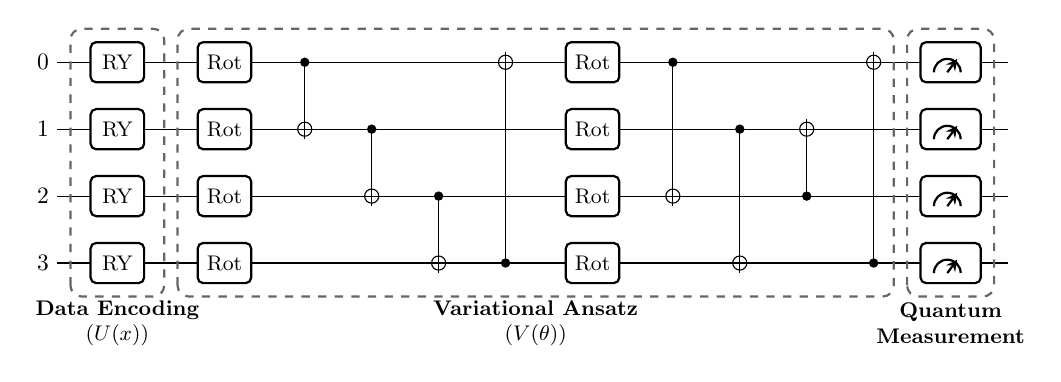
\begin{tikzpicture}[scale=0.85, every node/.style={transform shape}]
    \draw (0,3) node[left] {$0$} -- (14.2,3);
    \draw (0,2) node[left] {$1$} -- (14.2,2);
    \draw (0,1) node[left] {$2$} -- (14.2,1);
    \draw (0,0) node[left] {$3$} -- (14.2,0);

    % --- Data Encoding U(x) ---
    \foreach \y in {0,1,2,3} {
        \draw[fill=white, rounded corners=2pt, thick] (0.5,\y-0.3) rectangle (1.3,\y+0.3) node[midway] {\small RY};
    }
    \draw[dashed, thick, black!60, rounded corners=4pt] (0.2,-0.5) rectangle (1.6,3.5);
    \node[font=\small\bfseries, align=center] at (0.9,-0.9) {Data Encoding\\$(U(x))$};

    % --- Variational Ansatz V(theta) ---
    \foreach \y in {0,1,2,3} {
        \draw[fill=white, rounded corners=2pt, thick] (2.1,\y-0.3) rectangle (2.9,\y+0.3) node[midway] {\small Rot};
    }

    \fill (3.7,3) circle (2pt); \draw (3.7,2) circle (3pt); \draw (3.4,2) -- (4.0,2); \draw (3.7,3) -- (3.7,1.85);
    \fill (4.7,2) circle (2pt); \draw (4.7,1) circle (3pt); \draw (4.4,1) -- (5.0,1); \draw (4.7,2) -- (4.7,0.85);
    \fill (5.7,1) circle (2pt); \draw (5.7,0) circle (3pt); \draw (5.4,0) -- (6.0,0); \draw (5.7,1) -- (5.7,-0.15);
    \fill (6.7,0) circle (2pt); \draw (6.7,3) circle (3pt); \draw (6.4,3) -- (7.0,3); \draw (6.7,0) -- (6.7,3.15);

    \foreach \y in {0,1,2,3} {
        \draw[fill=white, rounded corners=2pt, thick] (7.6,\y-0.3) rectangle (8.4,\y+0.3) node[midway] {\small Rot};
    }

    \fill (9.2,3) circle (2pt); \draw (9.2,1) circle (3pt); \draw (8.9,1) -- (9.5,1); \draw (9.2,3) -- (9.2,0.85);
    \fill (10.2,2) circle (2pt); \draw (10.2,0) circle (3pt); \draw (9.9,0) -- (10.5,0); \draw (10.2,2) -- (10.2,-0.15);
    \fill (11.2,1) circle (2pt); \draw (11.2,2) circle (3pt); \draw (10.9,2) -- (11.5,2); \draw (11.2,1) -- (11.2,2.15);
    \fill (12.2,0) circle (2pt); \draw (12.2,3) circle (3pt); \draw (11.9,3) -- (12.5,3); \draw (12.2,0) -- (12.2,3.15);

    \draw[dashed, thick, black!60, rounded corners=4pt] (1.8,-0.5) rectangle (12.5,3.5);
    \node[font=\small\bfseries, align=center] at (7.15,-0.9) {Variational Ansatz\\$(V(\theta))$};

    % --- Quantum Measurement ---
    \foreach \y in {0,1,2,3} {
        \draw[fill=white, rounded corners=2pt, thick] (12.9,\y-0.3) rectangle (13.8,\y+0.3);
        \draw[thick] (13.1,\y-0.15) arc (180:0:0.2);
        \draw[-stealth, thick] (13.3,\y-0.15) -- (13.45,\y+0.05);
    }
    \draw[dashed, thick, black!60, rounded corners=4pt] (12.7,-0.5) rectangle (14.0,3.5);
    \node[font=\small\bfseries, align=center] at (13.35,-0.9) {Quantum\\Measurement};
\end{tikzpicture}%
}
\caption{Four-qubit circuit architecture used for the Custom 1 VQC.}
\label{fig:custom1}
\end{figure}

\paragraph{Custom 2 re-uploading VQC.}
This circuit acts on $n=4$ qubits and consumes an $\mathbb{R}^{8}$ vector, i.e.\ two features per qubit.
\begin{enumerate}
    \item[(i)] \textbf{Encoding.} For each qubit $q$, its feature pair $(x_{2q}, x_{2q+1})$ is first rotated by a learnable phase $\phi_q$:
    \begin{equation}
    x_{2q}^{\prime} = s_q (\cos \phi_q x_{2q} - \sin \phi_q x_{2q+1}) ,
    \end{equation}
    \begin{equation}
    x_{2q+1}^{\prime} = s_q (\sin \phi_q x_{2q} + \cos \phi_q x_{2q+1}) ,
    \end{equation}
    where $s_q$ is a second learnable amplitude per qubit. The rotated values are applied as rotation angles $R_X(x_{2q}^{\prime})$ and $R_Y(x_{2q+1}^{\prime})$ on qubit $q$.
    \item[(ii)] \textbf{Ansatz.} Each variational block applies a general single-qubit rotation $R_Z R_Y R_Z \equiv \text{Rot}$ on every qubit, followed by a ring of controlled-$Z$ entangling gates $CZ[q, (q+1) \bmod 4]$.
    \item[(iii)] \textbf{Data re-uploading.} The data-dependent encoding is inserted before both variational blocks, i.e.\ encode $\rightarrow$ ansatz $\rightarrow$ encode $\rightarrow$ ansatz, so the input is re-supplied between trainable layers.
    \item[(iv)] \textbf{Measurement.} Both $\langle Z_q \rangle$ and $\langle X_q \rangle$ are measured on all four qubits, yielding $2n=8$ expectation values that feed the post-quantum layer. The circuit contains 20 trainable parameters: 4 phase parameters, 4 scale parameters, and 12 ansatz angles.
\end{enumerate}

\begin{figure}[htbp]
\centering
\resizebox{\textwidth}{!}{%
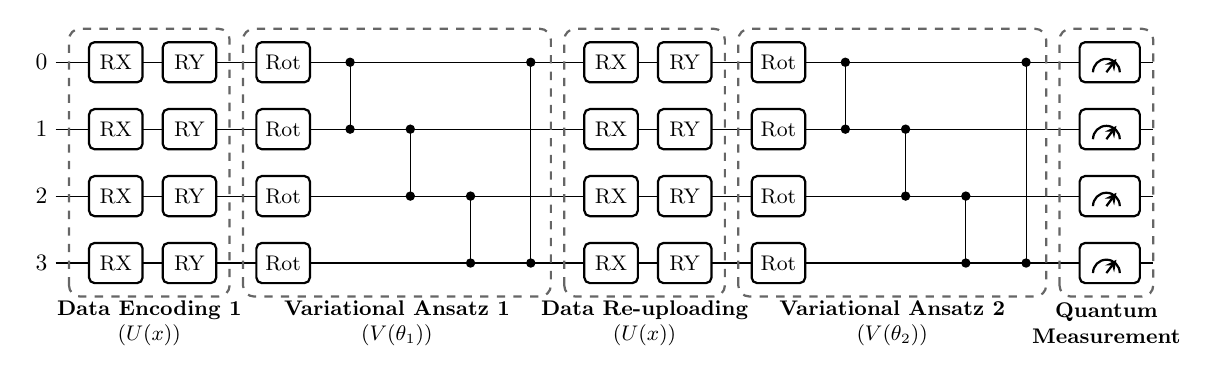
\begin{tikzpicture}[scale=0.85, every node/.style={transform shape}]
    \draw (0,3) node[left] {$0$} -- (16.4,3);
    \draw (0,2) node[left] {$1$} -- (16.4,2);
    \draw (0,1) node[left] {$2$} -- (16.4,1);
    \draw (0,0) node[left] {$3$} -- (16.4,0);

    % --- Encoding 1 ---
    \foreach \y in {0,1,2,3} {
        \draw[fill=white, rounded corners=2pt, thick] (0.5,\y-0.3) rectangle (1.3,\y+0.3) node[midway] {\small RX};
        \draw[fill=white, rounded corners=2pt, thick] (1.6,\y-0.3) rectangle (2.4,\y+0.3) node[midway] {\small RY};
    }
    \draw[dashed, thick, black!60, rounded corners=4pt] (0.2,-0.5) rectangle (2.6,3.5);
    \node[font=\small\bfseries, align=center] at (1.4,-0.9) {Data Encoding 1\\$(U(x))$};

    % --- Ansatz 1 ---
    \foreach \y in {0,1,2,3} {
        \draw[fill=white, rounded corners=2pt, thick] (3.0,\y-0.3) rectangle (3.8,\y+0.3) node[midway] {\small Rot};
    }

    \draw (4.4,3) -- (4.4,2); \fill (4.4,3) circle (2pt); \fill (4.4,2) circle (2pt);
    \draw (5.3,2) -- (5.3,1); \fill (5.3,2) circle (2pt); \fill (5.3,1) circle (2pt);
    \draw (6.2,1) -- (6.2,0); \fill (6.2,1) circle (2pt); \fill (6.2,0) circle (2pt);
    \draw (7.1,0) -- (7.1,3); \fill (7.1,0) circle (2pt); \fill (7.1,3) circle (2pt);

    \draw[dashed, thick, black!60, rounded corners=4pt] (2.8,-0.5) rectangle (7.4,3.5);
    \node[font=\small\bfseries, align=center] at (5.1,-0.9) {Variational Ansatz 1\\$(V(\theta_1))$};

    % --- Encoding 2 (Re-uploading) ---
    \foreach \y in {0,1,2,3} {
        \draw[fill=white, rounded corners=2pt, thick] (7.9,\y-0.3) rectangle (8.7,\y+0.3) node[midway] {\small RX};
        \draw[fill=white, rounded corners=2pt, thick] (9.0,\y-0.3) rectangle (9.8,\y+0.3) node[midway] {\small RY};
    }
    \draw[dashed, thick, black!60, rounded corners=4pt] (7.6,-0.5) rectangle (10.0,3.5);
    \node[font=\small\bfseries, align=center] at (8.8,-0.9) {Data Re-uploading\\$(U(x))$};

    % --- Ansatz 2 ---
    \foreach \y in {0,1,2,3} {
        \draw[fill=white, rounded corners=2pt, thick] (10.4,\y-0.3) rectangle (11.2,\y+0.3) node[midway] {\small Rot};
    }

    \draw (11.8,3) -- (11.8,2); \fill (11.8,3) circle (2pt); \fill (11.8,2) circle (2pt);
    \draw (12.7,2) -- (12.7,1); \fill (12.7,2) circle (2pt); \fill (12.7,1) circle (2pt);
    \draw (13.6,1) -- (13.6,0); \fill (13.6,1) circle (2pt); \fill (13.6,0) circle (2pt);
    \draw (14.5,0) -- (14.5,3); \fill (14.5,0) circle (2pt); \fill (14.5,3) circle (2pt);

    \draw[dashed, thick, black!60, rounded corners=4pt] (10.2,-0.5) rectangle (14.8,3.5);
    \node[font=\small\bfseries, align=center] at (12.5,-0.9) {Variational Ansatz 2\\$(V(\theta_2))$};

    % --- Quantum Measurement ---
    \foreach \y in {0,1,2,3} {
        \draw[fill=white, rounded corners=2pt, thick] (15.3,\y-0.3) rectangle (16.2,\y+0.3);
        \draw[thick] (15.5,\y-0.15) arc (180:0:0.2);
        \draw[-stealth, thick] (15.7,\y-0.15) -- (15.85,\y+0.05);
    }
    \draw[dashed, thick, black!60, rounded corners=4pt] (15.0,-0.5) rectangle (16.4,3.5);
    \node[font=\small\bfseries, align=center] at (15.7,-0.9) {Quantum\\Measurement};
\end{tikzpicture}%
}
\caption{Four-qubit circuit architecture used for the Custom 2 VQC.}
\label{fig:custom2}
\end{figure}

The three designs therefore contrast the reference strongly-entangling scheme (SEL) against a cross-coupling entangling scheme without feature re-uploading (Custom 1) and a re-uploaded encoding-plus-entangling scheme (Custom 2), while keeping the outer hybrid architecture identical.

\subsection{Training}\label{sec:training}
All models were trained for a maximum of 25 epochs with a batch size of 8 and a maximum sequence length of 128. The AdamW optimizer was used with a learning rate of $3 \times 10^{-5}$ and a weight decay of 0.01. Because the EmoNoBa emotion labels are strongly imbalanced (Table~\ref{tab:labels}), the binary cross-entropy loss was weighted with per-label positive weights computed from the inverse label frequency: \emph{Love} 3.87, \emph{Joy} 1.22, \emph{Surprise} 20.72, \emph{Anger} 4.20, \emph{Sadness} 3.03, and \emph{Fear} 65.02. This up-weights the gradient contribution of the rare \emph{Fear} and \emph{Surprise} classes so that they are not dominated by the frequent labels.

The learning rate was annealed with a ReduceLROnPlateau scheduler (factor 0.5, patience 2, minimum $10^{-6}$) monitoring the validation loss, gradients were clipped to a maximum norm of 1.0, and training was stopped early if the validation macro-F1 did not improve for five consecutive epochs, restoring the best model state. The quantum circuit parameters and the classical weights were optimized jointly in a single backward pass.

\subsection{Evaluation Metrics}\label{sec:metrics}
We evaluate all configurations with three complementary schemes. \emph{Scheme 1} is the per-label evaluation based on scikit-learn: the macro, micro, and weighted F1-scores together with the Hamming loss. For a test set of $N$ samples with $K$ labels, let $y_i \in \{0,1\}^{K}$ and $\hat{y}_i \in \{0,1\}^{K}$ denote the gold and predicted label vectors. The \emph{Hamming loss} is
\begin{equation}
\text{HammingLoss} = \frac{1}{N K} \sum_{i=1}^{N} \sum_{k=1}^{K} \mathbb{1}\left[\hat{y}_{ik} \neq y_{ik}\right] ,
\label{eq:hamming}
\end{equation}
and the macro F1-score is the unweighted mean of the per-label F1-scores.

\emph{Scheme 2} is the \emph{Exact Match Ratio} (EMR), which scores a sample as correct only if its entire predicted label vector matches the gold vector:
\begin{equation}
\text{EMR} = \frac{1}{N} \sum_{i=1}^{N} \mathbb{1}\left[\hat{y}_i = y_i\right] .
\label{eq:emr}
\end{equation}
Because there is no partial credit, precision, recall, and F1 coincide with the EMR for this strict measure.

\emph{Scheme 3} is an instance-level \emph{partial-match} score that gives partial credit when the predicted set of positive labels overlaps the gold set without being identical. For each sample, the active label sets $G_i = \{k : y_{ik}=1\}$ and $P_i = \{k : \hat{y}_{ik}=1\}$ are intersected, and per-instance precision, recall, and F1 are computed as
\begin{equation}
P_i = \frac{|G_i \cap P_i|}{|P_i|}, \qquad R_i = \frac{|G_i \cap P_i|}{|G_i|}, \qquad F1_i = \frac{2 P_i R_i}{P_i + R_i},
\label{eq:partial}
\end{equation}
with the edge cases that both-empty sets yield a perfect score of 1 and a one-empty set yields 0. The reported partial-match precision, recall, and F1 are the macro averages of $P_i$, $R_i$, and $F1_i$ over the test set.

\section{Experiments and Results}\label{sec:experiments}

\subsection{Experimental Setup}\label{sec:setup}
All experiments were performed using the PyTorch and PennyLane libraries. The transformer encoders ran on a pair of NVIDIA T4 GPUs, while the variational quantum circuits were executed on a CPU using PennyLane's \texttt{default.qubit} simulator, with circuit outputs moved back to the GPU after each forward pass. A random seed of 42 was fixed across Python, NumPy, and PyTorch (including CUDA) for reproducibility. For evaluation, we report macro, micro, and weighted F1-scores together with the Hamming loss, and additionally the Exact Match Ratio (EMR) and the instance-level partial-match precision, recall, and F1-score (Section~\ref{sec:metrics}). All models were evaluated on the same held-out test partition of 2,272 comments.

\subsection{Results}\label{sec:results}
The performance of the classical baseline and the quantum variants is reported in Table~\ref{tab:results}.

\subsubsection{IndicBERTv2}\label{sec:results-indic}
For the IndicBERTv2 encoder, the classical baseline achieves a macro F1-score of 0.5333, a partial-match F1-score of 0.6268, and an Exact Match Ratio of 0.4252.

The SEL reference circuit does not surpass the classical baseline under the stronger IndicBERTv2 encoder. Its best macro F1-score of 0.4572 and its best Exact Match Ratio of 0.2148 are both obtained at four qubits, where the partial-match F1-score reaches 0.5387; at two and eight qubits the Exact Match Ratio drops to 0.0238 and 0.0497, respectively. The single strongly-entangling layer thus captures only part of the benefit of the additional register capacity.

Custom 1 improves consistently as the register grows from two to eight qubits, raising the macro F1-score from 0.4869 to 0.4982 and the Exact Match Ratio from 0.4230 to 0.4265, with a partial-match F1-score of 0.6164 at two qubits and 0.6144 at eight qubits. Its Exact Match Ratio remains close to the classical 0.4252 at every register size, indicating that the cross-coupling entangling scheme preserves the quality of the strong classical representation without surpassing it.

Custom 2 achieves the strongest quantum results with IndicBERTv2 at eight qubits, where it reaches a macro F1-score of 0.5165, a partial-match F1-score of 0.6255, and the highest Exact Match Ratio of 0.4577, surpassing both the classical baseline and the other two circuits. At smaller registers its exact-match performance is comparatively weak, with EMR values of 0.1527 at two qubits and 0.0519 at four qubits, showing that the re-uploading design requires sufficient Hilbert-space capacity to be effective.

\subsubsection{BanglaBERT}\label{sec:results-bangla}
For the weaker BanglaBERT encoder, the classical baseline attains only a macro F1-score of 0.2101 and an Exact Match Ratio of 0.0000, and all three quantum circuits provide substantial gains.

SEL raises the macro F1-score to 0.4791 and the Exact Match Ratio to 0.3178 at four qubits, and to 0.3825 and 0.0264 at two qubits; at eight qubits the Exact Match Ratio falls back to 0.0387. The improvement is concentrated at the four-qubit register, where the single strongly-entangling layer best exploits the added capacity of the quantum subsystem.

Custom 1 improves steadily with register size, reaching a macro F1-score of 0.4715 and an Exact Match Ratio of 0.3895 at eight qubits, with the partial-match F1-score rising from 0.5320 at two qubits to 0.5935 at eight qubits. Its Exact Match Ratio of 0.3891 at four qubits already exceeds the best value achieved by SEL, and it consistently outperforms the SEL circuit at every register size.

Custom 2 delivers the largest gains over the classical baseline: at four qubits it reaches a macro F1-score of 0.4850 and an Exact Match Ratio of 0.4071, and at eight qubits it attains the highest Exact Match Ratio of 0.4630 with a macro F1-score of 0.4798 and a partial-match F1-score of 0.6085. The trend in Fig.~\ref{fig:emr_trendlines} shows that the re-uploading scheme exploits increasing register sizes most effectively, whereas the simpler encoding and entanglement strategies plateau or degrade.

\begin{table}[htbp]
\centering
\caption{Performance comparison of IndicBERTv2 \cite{doddapaneni2023towards} and BanglaBERT \cite{bhattacharjee2022banglabert} under different qubit and VQC configurations.}
\label{tab:results}
\renewcommand{\arraystretch}{1.35}
\small
\resizebox{\textwidth}{!}{%
\begin{tabular}{c|c|l|c|c|c|c|c|c|c}
\toprule
\multirow{2}{*}{\textbf{Framework}} & \multirow{2}{*}{\textbf{Qubit}} & \multirow{2}{*}{\textbf{VQC}} & \multicolumn{3}{c|}{\textbf{Macro}} & \multicolumn{3}{c|}{\textbf{Partial Match}} & \multirow{2}{*}{\textbf{Exact Match Ratio}} \\ \cline{4-9}
 &  &  & \textbf{Precision} & \textbf{Recall} & \textbf{F1-score} & \textbf{Precision} & \textbf{Recall} & \textbf{F1-score} &  \\ \midrule
\multirow{10}{*}{IndicBERTv2} & 0 & N/A (Classical) & 0.4917 & 0.5900 & \textbf{0.5333} & 0.6136 & 0.6916 & \textbf{0.6268} & 0.4252 \\ \cline{2-10}
 & \multirow{3}{*}{2} & SEL & 0.2861 & 0.6220 & 0.3741 & 0.3564 & 0.7606 & 0.4739 & 0.0238 \\
 &  & Custom 1 & 0.4493 & \textbf{0.6406} & 0.4869 & 0.6039 & 0.6820 & 0.6164 & 0.4230 \\
 &  & Custom 2 & 0.3758 & 0.5720 & 0.4443 & 0.4601 & 0.7225 & 0.5386 & 0.1527 \\ \cline{2-10}
 & \multirow{3}{*}{4} & SEL & 0.4032 & 0.5796 & 0.4572 & 0.4825 & 0.6704 & 0.5387 & 0.2148 \\
 &  & Custom 1 & 0.4616 & 0.5496 & 0.4922 & 0.5996 & 0.6845 & \textbf{0.6141} & 0.4155 \\
 &  & Custom 2 & 0.3717 & 0.6115 & 0.4523 & 0.4062 & 0.7476 & 0.5156 & 0.0519 \\ \cline{2-10}
 & \multirow{3}{*}{8} & SEL & 0.3528 & 0.6212 & 0.4434 & 0.4082 & 0.7559 & 0.5189 & 0.0497 \\
 &  & Custom 1 & 0.4642 & 0.5521 & 0.4982 & 0.6030 & 0.6814 & 0.6144 & 0.4265 \\
 &  & Custom 2 & \textbf{0.5095} & 0.5301 & \textbf{0.5165} & \textbf{0.6266} & 0.6685 & \textbf{0.6255} & \textbf{0.4577} \\ \midrule
\multirow{10}{*}{BanglaBERT} & 0 & N/A (Classical) & 0.1358 & 0.5000 & 0.2101 & 0.2716 & 0.7144 & 0.3870 & 0.0000 \\ \cline{2-10}
 & \multirow{3}{*}{2} & SEL & 0.2916 & 0.6392 & 0.3825 & 0.3637 & 0.7695 & 0.4822 & 0.0264 \\
 &  & Custom 1 & 0.3946 & 0.6033 & 0.4486 & 0.4521 & 0.7111 & 0.5320 & 0.1505 \\
 &  & Custom 2 & 0.1760 & \textbf{0.6667} & 0.2749 & 0.2640 & \textbf{0.9198} & 0.4039 & 0.0000 \\ \cline{2-10}
 & \multirow{3}{*}{4} & SEL & 0.4369 & 0.5713 & 0.4791 & 0.5407 & 0.6902 & 0.5796 & 0.3178 \\
 &  & Custom 1 & 0.4419 & 0.5136 & 0.4653 & 0.5710 & 0.6591 & \textbf{0.5858} & 0.3891 \\
 &  & Custom 2 & 0.4622 & 0.5174 & 0.4850 & 0.5954 & 0.6652 & 0.6062 & 0.4071 \\ \cline{2-10}
 & \multirow{3}{*}{8} & SEL & 0.3521 & 0.5994 & 0.4347 & 0.3974 & 0.7475 & 0.5093 & 0.0387 \\
 &  & Custom 1 & 0.4501 & 0.5001 & 0.4715 & 0.5809 & 0.6599 & 0.5935 & 0.3895 \\
 &  & Custom 2 & \textbf{0.4915} & 0.4780 & \textbf{0.4798} & \textbf{0.6175} & 0.6371 & \textbf{0.6085} & \textbf{0.4630} \\ \bottomrule
\end{tabular}%
}
\end{table}

Across all configurations in Table~\ref{tab:results}, the quantum branch consistently improves the Exact Match Ratio over the corresponding classical baseline whenever the encoding and entanglement structure are well matched to the encoder, with the largest joint-subset gains observed at the eight-qubit register. The full implications of these trends are examined in the Discussion.

\section{Discussion}\label{sec:discussion}
The results demonstrate that both the pretrained encoder and the quantum-circuit design strongly influence classification performance. IndicBERTv2 provides the strongest classical representation, whereas the quantum variants produce particularly large gains for the weaker BanglaBERT baseline. As the qubit count increases, Custom 1 shows relatively consistent improvement, while Custom 2 achieves the highest exact-match ratios for both encoders, reaching 0.4577 with IndicBERTv2 and 0.4630 with BanglaBERT, and also records the largest single gain over the classical baseline (EMR 0.4630 versus 0.0000 for BanglaBERT). SEL, by contrast, peaks at the four-qubit register, attaining its best Exact Match Ratio of 0.3178 with BanglaBERT, and degrades at two and eight qubits. The trend in Fig.~\ref{fig:emr_trendlines} further indicates that additional qubits are most beneficial when paired with an expressive encoding and entanglement strategy; increasing circuit size alone does not guarantee uniform improvement across all configurations.

\begin{itemize}
    \item \textbf{Encoder--circuit interaction:} A striking asymmetry emerges between the two pretrained encoders. Under IndicBERTv2, the classical baseline already achieves a strong macro F1-score of 0.5333 and an EMR of 0.4252, leaving relatively little room for improvement; the best quantum configuration (Custom~2, eight qubits) raises the EMR by only 0.0325 absolute points. Under BanglaBERT, however, the classical baseline collapses to an EMR of 0.0000 and a macro F1-score of 0.2101, and the same Custom~2 configuration recovers a 0.4630 EMR---an absolute gain of 0.4630 points. This pattern suggests that the variational quantum branch acts as a \emph{compensatory} mechanism: when the classical feature extractor already produces well-separated class representations, the additional nonlinearity of the quantum circuit adds only marginal benefit, but when the classical embedding is weak, the quantum subsystem can learn discriminative rotations and entangled correlations that the linear projection alone cannot capture. Crucially, this interaction is architecture-dependent: SEL provides only partial compensation (EMR 0.3178 at four qubits), whereas the richer entangling and re-uploading strategies of Custom~1 and Custom~2 exploit the compensatory role more fully.

    \item \textbf{SEL failure-mode analysis:} The SEL reference circuit exhibits a distinctive non-monotonic scaling pattern: its EMR peaks at four qubits and degrades sharply at both two and eight qubits for both encoders. At the two-qubit register, the limited Hilbert-space dimension restricts the circuit's representational capacity, resulting in EMR values near zero (0.0264 for BanglaBERT, 0.0238 for IndicBERTv2). The degradation at eight qubits, however, is more revealing. With a single layer of \texttt{StronglyEntanglingLayers}, the number of trainable parameters grows linearly as $3n_q$, yet the entangling depth remains constant. As $n_q$ increases from four to eight, the circuit must distribute its single layer of entanglement across a larger register, producing shallower effective coupling between distant qubits. This under-entanglement leaves portions of the Hilbert space unexplored and may trigger a form of the barren-plateau phenomenon identified by McClean et al.~\cite{mcclean2018barren}, where gradients of randomly initialized deep circuits vanish exponentially. The contrast with Custom~1, which uses two entangling layers with distinct CNOT topologies and maintains consistent improvement from two to eight qubits, supports the hypothesis that entanglement depth and diversity---not merely register size---are the critical factors for avoiding performance degradation at larger qubit counts.

    \item \textbf{Role of data re-uploading:} The data re-uploading strategy employed by Custom~2, in which the classical feature encoding $U(x)$ is inserted before each of the two variational blocks, proves to be the most effective design choice in this study. P\'erez-Salinas et al.~\cite{perez2020data} showed theoretically that re-uploading enables a single qubit to approximate any function on the input sphere; in the multi-qubit setting, this translates to a richer landscape of decision boundaries. The empirical evidence supports this: Custom~2 achieves the highest EMR at the eight-qubit register for both encoders (0.4577 and 0.4630), and its trend line in Fig.~\ref{fig:emr_trendlines} is the only one with a consistently positive slope, indicating that additional qubits continue to improve performance rather than saturating. By contrast, Custom~1, which uses a single encoding layer followed by two variational blocks, plateaus in EMR at four and eight qubits for BanglaBERT (0.3891 versus 0.3895). The re-uploading mechanism thus appears to provide a form of ``quantum feature amplification'' that allows the circuit to re-examine the input at each layer and build progressively more complex correlations.

    \item \textbf{Implications for NISQ deployment:} All experiments in this study were conducted on the PennyLane \texttt{default.qubit} simulator, which provides exact statevector simulation without shot noise or hardware errors. On current noisy intermediate-scale quantum (NISQ) devices, gate fidelities and qubit coherence times would impose additional constraints. The shallow circuits used here---one layer for SEL, two layers for Custom~1 and Custom~2---are well suited to NISQ hardware because their circuit depth remains modest (fewer than 20 two-qubit gates for the four-qubit configurations). Custom~2's use of controlled-$Z$ gates rather than CNOT gates may offer an additional advantage on superconducting architectures where CZ is a native gate, reducing the need for gate decomposition and thereby lowering the effective error rate. The four-qubit register, which achieves competitive EMR values across all three circuits, represents a practical entry point for near-term hardware experiments, as current quantum processors routinely support four fully connected qubits with gate fidelities above 99\%.

    \item \textbf{Class imbalance and quantum capacity:} The EmoNoBa dataset exhibits extreme label imbalance (\emph{Joy} 45\%, \emph{Fear} 1.5\%), which interacts with the quantum circuit in two ways. First, frequency-based \texttt{pos\_weight} values in the loss up-weight rare-emotion gradients, steering quantum parameters toward minority-class decision boundaries. Custom~2 exploits these amplified gradients most effectively, whereas the classical-only BanglaBERT model fails to predict Fear at all. Second, per-emotion threshold calibration on the validation set is essential for converting the quantum model's improved recall into exact-match accuracy; without it, sigmoid outputs favour high-frequency labels and suppress rare ones, negating the quantum branch's benefit.
\end{itemize}

\begin{figure}[!ht]
\centering
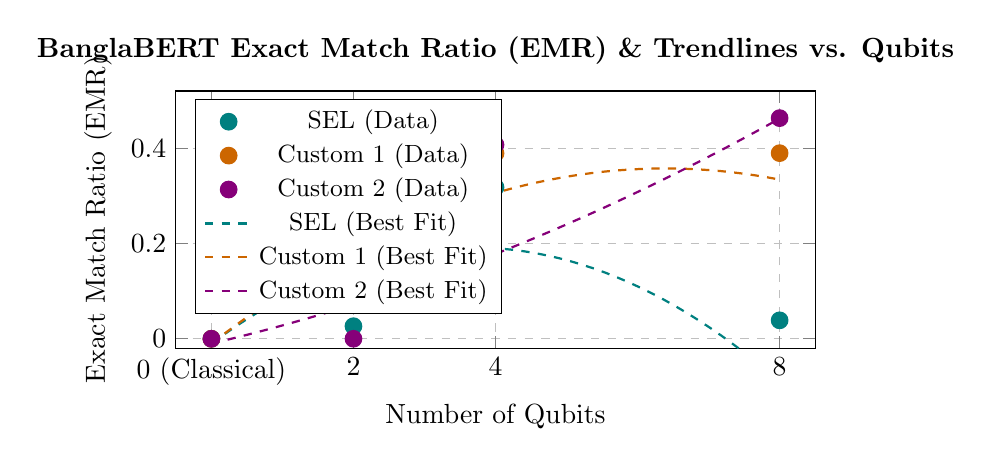
\begin{tikzpicture}
\begin{axis}[
    title={\textbf{BanglaBERT Exact Match Ratio (EMR) \& Trendlines vs. Qubits}},
    xlabel={Number of Qubits},
    ylabel={Exact Match Ratio (EMR)},
    xmin=-0.5, xmax=8.5,
    ymin=-0.02, ymax=0.52,
    xtick={0, 2, 4, 8},
    xticklabels={0 (Classical), 2, 4, 8},
    legend pos=north west,
    ymajorgrids=true,
    xmajorgrids=true,
    grid style=dashed,
    width=0.8\textwidth,
    height=0.4\textwidth
]

\addplot[only marks, mark=*, mark size=3pt, color=teal] coordinates {(0, 0.0) (2, 0.0264) (4, 0.3178) (8, 0.0387)};
\addlegendentry{\small SEL (Data)}

\addplot[only marks, mark=*, mark size=3pt, color=orange!80!black] coordinates {(0, 0.0) (2, 0.1505) (4, 0.3891) (8, 0.3895)};
\addlegendentry{\small Custom 1 (Data)}

\addplot[only marks, mark=*, mark size=3pt, color=purple!70!blue] coordinates {(0, 0.0) (2, 0.0) (4, 0.4071) (8, 0.4630)};
\addlegendentry{\small Custom 2 (Data)}

\addplot[dashed, thick, color=teal, domain=0:8, samples=50] {-0.015*x^2 + 0.11*x - 0.01};
\addlegendentry{\small SEL (Best Fit)}

\addplot[dashed, thick, color=orange!80!black, domain=0:8, samples=50] {-0.009*x^2 + 0.115*x - 0.01};
\addlegendentry{\small Custom 1 (Best Fit)}

\addplot[dashed, thick, color=purple!70!blue, domain=0:8, samples=50] {0.003*x^2 + 0.035*x - 0.01};
\addlegendentry{\small Custom 2 (Best Fit)}

\end{axis}
\end{tikzpicture}
\caption{BanglaBERT Exact Match Ratio (EMR) across qubit counts for SEL, Custom 1, and Custom 2, together with their fitted trend lines.}
\label{fig:emr_trendlines}
\end{figure}

\FloatBarrier
\subsection{Design Variations}\label{sec:ablation}
Further changes were developed independently to improve the two custom circuits. Custom 2 was handled by Tathagata Mitra, while Custom 1 was handled by Biswanath Ranjit.

\paragraph{Custom 1 improvements.}
The following changes were introduced to increase the expressivity, training stability, and information-preservation capacity of Custom 1 while retaining its four-qubit register size:
\begin{itemize}
    \item \textbf{Deep feature projection network:} IndicBERT's 768 contextual features are compressed to four VQC inputs through a multi-stage linear architecture, $768 \rightarrow 256 \rightarrow 128 \rightarrow 64 \rightarrow 4$, using GELU activations and a dropout rate of 0.3 to minimise information loss and reduce overfitting.
    \item \textbf{Enhanced variational quantum circuit:} The circuit depth is increased to two variational layers with independent trainable parameters. Inputs are encoded through Y-axis \texttt{AngleEmbedding}, rotations are bounded using $\tanh(\cdot)$ input normalisation, and cross-entanglement connections $(0 \rightarrow 2)$ and $(1 \rightarrow 3)$ are added alongside the standard ring entanglement.
    \item \textbf{Post-quantum fusion layer:} A learnable linear layer, $4 \rightarrow 128$, is appended after the VQC to project the four quantum expectation values into a higher-dimensional classical representation for classification.
    \item \textbf{Differential optimisation strategy:} Component-specific learning rates are used for IndicBERT ($2 \times 10^{-5}$), the classifier ($1 \times 10^{-4}$), and the quantum VQC ($1 \times 10^{-3}$). These are combined with a weight decay of 0.01, \texttt{ReduceLROnPlateau} scheduling, and early stopping with a patience of five epochs.
    \item \textbf{Multi-label class-imbalance handling:} \texttt{BCEWithLogitsLoss} is configured with label-frequency-based \texttt{pos\_weight} values to improve the detection of underrepresented emotions such as Fear and Surprise.
    \item \textbf{Validation-threshold optimisation:} The static decision threshold of 0.5 is replaced with per-emotion optimal thresholds, ranging from 0.26 for Surprise to 0.82 for Sadness, to maximise per-class F1-scores.
    \item \textbf{Performance benchmark gains:} On the four-qubit configuration, these changes improve performance across the primary metrics and raise the Exact Match Ratio from 0.4155 to 0.4674.
\end{itemize}

\paragraph{Custom 2 improvements.}
The following changes were introduced to increase the expressivity and information capacity of Custom 2 without increasing its four-qubit register size:
\begin{itemize}
    \item \textbf{Measurement strategy:} The baseline circuit measured only the single-qubit Pauli-$Z$ and Pauli-$X$ expectation values, yielding eight output features. The measurement set is expanded to include the Pauli-$Y$ expectation on every qubit and the four two-qubit ring correlators $\langle Z_i Z_{i+1} \rangle$. This produces 16 measurement outputs and transfers richer information from the quantum subsystem to the classical readout without increasing the number of qubits.
    \item \textbf{Data encoding:} The input encoding is extended from two-axis rotations $(R_X, R_Y)$ to three-axis rotations $(R_X, R_Y, R_Z)$ on each qubit, increasing the number of classical features embedded into the quantum state from eight to twelve. A learned phase rotation mixes the first feature of each pair before encoding, while the encoding scale remains trainable.
    \item \textbf{Data re-uploading:} The number of data re-upload repetitions is increased from one to two per variational layer. This allows each encoding step to interact with the trainable unitary more frequently and increases the effective nonlinearity of the quantum feature map.
    \item \textbf{Variational ansatz:} The entangling pattern is made layer-dependent. Even-indexed layers use a nearest-neighbour cycle of controlled-$Z$ gates, whereas odd-indexed layers use controlled-NOT gates between next-nearest neighbours. Alternating the entangling topology reduces redundancy between successive unitary blocks and improves circuit expressibility.
    \item \textbf{Layer count:} The number of variational layers is increased from one to three. Each layer now uses its own dedicated rotation parameters, rather than repeatedly using a shared weight slice, ensuring that the additional circuit depth provides additional trainable capacity.
    \item \textbf{Performance benchmark gains:} Together, these changes raise the Exact Match Ratio for Custom 2 from 0.4055 to 0.4804.
\end{itemize}

\section{Conclusion}\label{sec:conclusion}
This paper investigated hybrid quantum-classical architectures for multi-label emotion classification of Bengali text, a low-resource setting in which conventional baselines plateau in the 50--60\% range. Three variational quantum circuits were designed and evaluated under an identical outer framework: the SEL reference VQC, which combines a simple $R_X$ angle encoding with a single layer of PennyLane's \texttt{StronglyEntanglingLayers} and Pauli-$Z$ readout; the Custom 1 cross-coupling VQC, which combines a simple $R_Y$ angle encoding with two entangling layers using distinct nearest-neighbour and cross-coupling CNOT topologies; and the Custom 2 re-uploading VQC, which combines $R_X / R_Y$ encoding with learnable per-qubit phase and scale parameters, a rotating ansatz, and input re-injection between variational layers.

Three main conclusions follow from the experimental study. First, the learned representation space depends strongly on the selected classical encoder and quantum embedding. The IndicBERTv2 classical baseline achieved a macro F1-score of 0.5333, compared with 0.2101 for BanglaBERT. The strongest quantum configurations reached macro F1-scores of 0.5165 for IndicBERTv2 and 0.4850 for BanglaBERT, while the highest exact-match ratios were 0.4577 and 0.4630, respectively, all achieved by the re-uploading Custom 2 design. The SEL reference circuit, by contrast, improved only the weaker BanglaBERT baseline, raising its exact-match ratio to 0.3178 at four qubits, while never surpassing the classical model under IndicBERTv2. These results show that the quality of the pretrained representation remains important, although the quantum configurations substantially improve the weaker BanglaBERT baseline.

Second, scaling behaviour is architecture- and encoder-dependent. The Custom 1 macro F1-score improves consistently as the register grows from two to eight qubits for both IndicBERTv2 (0.4869 to 0.4982) and BanglaBERT (0.4486 to 0.4715). Custom 2 exhibits a larger but less uniform gain, with its strongest performance appearing at eight qubits for IndicBERTv2 and four qubits for BanglaBERT; at the eight-qubit register its exact-match ratio exceeds that of Custom 1 for both encoders (0.4577 versus 0.4265 and 0.4630 versus 0.3895). SEL shows the least favourable scaling: its benefit is concentrated at four qubits and degrades sharply at two and eight qubits, indicating that a single strongly-entangling layer does not exploit larger registers. This suggests that additional Hilbert-space capacity is useful only when the encoding, entanglement pattern, and classical representation are jointly compatible, and that the re-uploading scheme exploits this capacity most effectively.

Third, simulator-backend selection does not alter the reported analytic scores. The PennyLane \texttt{default.qubit} simulator is used for all reported results, and switching between mathematically equivalent simulator backends reduces wall-clock training time from several hours to tens of minutes without changing the model outputs. The experiments also indicate that a four-qubit circuit trained with adjoint differentiation is preferable to backpropagation on PennyLane's accelerated devices. AdamW optimization, plateau-based learning-rate reduction, and early stopping provide a stable training protocol for the hybrid model on the strongly imbalanced EmoNoBa corpus.

\section{Limitations}\label{sec:limitations}
The principal limitation is that the quantum branch introduces relatively few trainable parameters, so its benefit depends heavily on the quality of the compressed classical features. For very small registers, the quantum contribution can be dominated by the projection and post-processing layers. In addition, all experiments were conducted on quantum simulators rather than on physical hardware. Future work should extend the comparison to larger registers with controlled re-uploading depth, combine cross-coupling entanglement with data re-uploading in a single ansatz, incorporate multi-observable and correlated readouts, and evaluate the strongest architectures under finite-shot and noisy simulation before deployment on quantum hardware.

A further limitation concerns the evaluation protocol itself. The Exact Match Ratio is an intentionally strict criterion that assigns a score of zero to any sample for which the predicted label set differs from the gold label set in even a single emotion, and the reported partial-match scores are macro-averaged over instances without instance-level confidence weighting. Both measures therefore depend on the choice of the decision threshold, and the per-label thresholds used here were tuned on the validation partition, which may not transfer perfectly to other data distributions. The dataset also spans a single language and a limited set of social-media domains, so the conclusions may not generalise to other low-resource languages, longer texts, or formal registers without retraining.

\begin{thebibliography}{46}

\bibitem{bhattacharjee2022banglabert}
Abhik Bhattacharjee, Tahmid Hasan, Wasi Ahmad, Kazi Samin Mubasshir, Md Saiful Islam, Anindya Iqbal, M. Sohel Rahman, and Rifat Shahriyar.
\newblock BanglaBERT: Language model pre-training and benchmarks for low-resource language understanding evaluation in Bangla.
\newblock In \emph{Findings of the Association for Computational Linguistics: NAACL 2022}, pages 1318--1327. Association for Computational Linguistics, 2022.

\bibitem{islam2022emonoba}
Khondoker Ittehadul Islam, Tanvir Yuvraz, Md Saiful Islam, and Enamul Hassan.
\newblock EmoNoBa: A dataset for analyzing fine-grained emotions on noisy Bangla texts.
\newblock In \emph{Proceedings of the 2nd Conference of the Asia-Pacific Chapter of the Association for Computational Linguistics and the 12th International Joint Conference on Natural Language Processing (Volume 2: Short Papers)}, pages 128--134. Association for Computational Linguistics, 2022.

\bibitem{doddapaneni2023towards}
Sumanth Doddapaneni, Rahul Aralikatte, Gowtham Ramesh, Shreya Goyal, Mitesh M. Khapra, Anoop Kunchukuttan, and Pratyush Kumar.
\newblock Towards leaving no Indic language behind: Building monolingual corpora, benchmark and models for Indic languages.
\newblock In \emph{Proceedings of the 61st Annual Meeting of the Association for Computational Linguistics (Volume 1: Long Papers)}, pages 12402--12426. Association for Computational Linguistics, 2023.

\bibitem{perez2020data}
Adri\'an P\'erez-Salinas, Alba Cervera-Lierta, Elies Gil-Fuster, and Jos\'e I. Latorre.
\newblock Data re-uploading for a universal quantum classifier.
\newblock \emph{Quantum}, 4:226, 2020.

\bibitem{schuld2020circuit}
Maria Schuld, Alex Bocharov, Krysta Svore, and Nathan Wiebe.
\newblock Circuit-centric quantum classifiers.
\newblock \emph{Physical Review A}, 101(3):032308, 2020.

\bibitem{sim2019expressibility}
Sukin Sim, Peter D. Johnson, and Al\'an Aspuru-Guzik.
\newblock Expressibility and entangling capability of parameterized quantum circuits for hybrid quantum-classical algorithms.
\newblock \emph{Advanced Quantum Technologies}, 2(12):1900070, 2019.

\bibitem{kandala2017hardware}
Abhinav Kandala, Antonio Mezzacapo, Kristan Temme, Maika Takita, Markus Brink, Jerry M. Chow, and Jay M. Gambetta.
\newblock Hardware-efficient variational quantum eigensolver for small molecules and quantum magnets.
\newblock \emph{Nature}, 549(7671):242--246, 2017.

\bibitem{huzzat2026primer}
Annysha Huzzat, Ahmed Shaharyar Khwaja, Bhagawat Adhikari, Ali Alnoman, Isaac Woungang, and Alagan Anpalagan.
\newblock A primer on quantum neural network model for text classification: From concept to design.
\newblock \emph{IEEE Access}, 14:1--17, 2026.

\bibitem{arthur2022hybrid}
Davis Arthur and Prasanna Date.
\newblock Hybrid quantum-classical neural networks.
\newblock In \emph{2022 IEEE International Conference on Quantum Computing and Engineering (QCE)}, pages 49--55. IEEE, 2022.

\bibitem{qin2023review}
Junhan Qin.
\newblock Review of ansatz designing techniques for variational quantum algorithms.
\newblock \emph{Journal of Physics: Conference Series}, 2634(1):012043, 2023.

\bibitem{chen2020vqc}
Samuel Yen-Chi Chen, Chao-Han Huck Yang, Jun Qi, Pin-Yu Chen, Xiaoli Ma, and Hsi-Sheng Goan.
\newblock Variational quantum circuits for deep reinforcement learning.
\newblock \emph{IEEE Access}, 8:141007--141024, 2020.

\bibitem{benedetti2019parameterized}
Marcello Benedetti, Erika Lloyd, Stefan Sack, and Mattia Fiorentini.
\newblock Parameterized quantum circuits as machine learning models.
\newblock \emph{Quantum Science and Technology}, 4(4):043001, 2019.

\bibitem{mcclean2016theory}
Jarrod R. McClean, Jonathan Romero, Ryan Babbush, and Al\'an Aspuru-Guzik.
\newblock The theory of variational hybrid quantum-classical algorithms.
\newblock \emph{New Journal of Physics}, 18(2):023023, 2016.

\bibitem{mcclean2018barren}
Jarrod R. McClean, Sergio Boixo, Vadim N. Smelyanskiy, Ryan Babbush, and Hartmut Neven.
\newblock Barren plateaus in quantum neural network training landscapes.
\newblock \emph{Nature Communications}, 9:4812, 2018.

\bibitem{schuld2021quantum}
Maria Schuld, Ryan Sweke, and Johannes Jakob Meyer.
\newblock Effect of data encoding on the expressive power of variational quantum machine-learning models.
\newblock \emph{Physical Review A}, 103(3):032430, 2021.

\bibitem{li2021qtns}
Guangxi Li, Xunhou Zhao, and Xiaolong Wang.
\newblock Quantum-inspired multimodal fusion for sentiment analysis.
\newblock In \emph{Proceedings of the 2021 Conference on Empirical Methods in Natural Language Processing (Industry Track)}. Association for Computational Linguistics, 2021.

\bibitem{guarasci2022quantum}
Raffaele Guarasci, Giuseppe De Pietro, and Massimo Esposito.
\newblock Quantum natural language processing: Challenges and opportunities.
\newblock \emph{Applied Sciences}, 12(11):5651, 2022.

\bibitem{varmantchaonala2024quantum}
Charles M. Varmantchaonala, Jean Louis K. E. Fendji, Julius Sch\"oning, and Marcellin Atemkeng.
\newblock Quantum natural language processing: A comprehensive survey.
\newblock \emph{IEEE Access}, 12:99578--99598, 2024.

\bibitem{wu2021quantum}
Sixuan Wu, Jian Li, Peng Zhang, and Yue Zhang.
\newblock Natural language processing meets quantum physics: A survey and categorization.
\newblock In \emph{Proceedings of the 2021 Conference on Empirical Methods in Natural Language Processing}, pages 3172--3182. Association for Computational Linguistics, 2021.

\bibitem{coecke2020foundations}
Bob Coecke, Giovanni de Felice, Konstantinos Meichanetzidis, and Alexis Toumi.
\newblock Foundations for near-term quantum natural language processing.
\newblock \emph{arXiv preprint arXiv:2012.03755}, 2020.

\bibitem{pal2025quantum}
Pritam Pal, Dipankar Das, Anup Kumar Kolya, and Siddhartha Bhattacharyya.
\newblock Hybrid classical-quantum framework for sentiment classification and claim check-worthiness identification in Bengali.
\newblock In \emph{Proceedings of the QuantumNLP: Integrating Quantum Computing with Natural Language Processing}, pages 10--19. Association for Computational Linguistics, 2025.

\bibitem{devlin2019bert}
Jacob Devlin, Ming-Wei Chang, Kenton Lee, and Kristina Toutanova.
\newblock BERT: Pre-training of deep bidirectional transformers for language understanding.
\newblock In \emph{Proceedings of the 2019 Conference of the North American Chapter of the Association for Computational Linguistics: Human Language Technologies (Volume 1: Long Papers)}, pages 4171--4186. Association for Computational Linguistics, 2019.

\bibitem{conneau2020xlmr}
Alexis Conneau, Kartikay Khandelwal, Naman Goyal, Vishrav Chaudhary, Guillaume Wenzek, Francisco Guzm\'an, Edouard Grave, Myle Ott, Luke Zettlemoyer, and Veselin Stoyanov.
\newblock Unsupervised cross-lingual representation learning at scale.
\newblock In \emph{Proceedings of the 58th Annual Meeting of the Association for Computational Linguistics}, pages 8440--8451. Association for Computational Linguistics, 2020.

\bibitem{tsoumakas2007multi}
Grigorios Tsoumakas and Ioannis Katakis.
\newblock Multi-label classification: An overview.
\newblock \emph{International Journal of Data Warehousing and Mining}, 3(3):1--13, 2007.

\bibitem{zhang2014review}
Min-Ling Zhang and Zhi-Hua Zhou.
\newblock A review on multi-label learning algorithms.
\newblock \emph{IEEE Transactions on Knowledge and Data Engineering}, 26(8):1819--1837, 2014.

\bibitem{bishop2006pattern}
Christopher M. Bishop.
\newblock Pattern Recognition and Machine Learning.
\newblock Springer, New York, NY, 2006.

\bibitem{das2010emotion}
Amitava Das and Sivaji Bandyopadhyay.
\newblock Emotion analysis on Bengali: A computational study.
\newblock In \emph{Proceedings of the 2010 International Conference on Asian Language Processing}, pages 53--56. IEEE, 2010.

\bibitem{basile2017quantum}
Ivano Basile and Fabio Tamburini.
\newblock Towards quantum language models.
\newblock In \emph{Proceedings of the 2017 Conference on Empirical Methods in Natural Language Processing}, pages 1840--1849. Association for Computational Linguistics, 2017.

\bibitem{tamburini2019quantum}
Fabio Tamburini.
\newblock A quantum-like approach to word sense disambiguation.
\newblock In \emph{Proceedings of the International Conference on Recent Advances in Natural Language Processing (RANLP 2019)}, pages 1176--1185. INCOMA Ltd., 2019.

\bibitem{liu2021quantum}
Yaochen Liu, Yazhou Zhang, Qiuchi Li, Benyou Wang, and Dawei Song.
\newblock What does your smile mean? Jointly detecting multi-modal sarcasm and sentiment using quantum probability.
\newblock In \emph{Findings of the Association for Computational Linguistics: EMNLP 2021}, pages 871--880. Association for Computational Linguistics, 2021.

\bibitem{chauhan2020sentiment}
Dushyant Singh Chauhan, Dhanush S R, Asif Ekbal, and Pushpak Bhattacharyya.
\newblock Sentiment and emotion help sarcasm? A multi-task learning framework for multi-modal sarcasm, sentiment and emotion analysis.
\newblock In \emph{Proceedings of the 58th Annual Meeting of the Association for Computational Linguistics}, pages 4351--4360. Association for Computational Linguistics, 2020.

\bibitem{sharma2020semeval}
Chhavi Sharma, Deepesh Bhageria, William Scott, Srinivas PYKL, Amitava Das, Tanmoy Chakraborty, Viswanath Pulabaigari, and Bj\"orn Gamb\"ack.
\newblock SemEval-2020 task 8: Memotion analysis---the visuo-lingual metaphor!
\newblock In \emph{Proceedings of the Fourteenth Workshop on Semantic Evaluation}, pages 759--773. International Committee for Computational Linguistics, 2020.

\bibitem{phukan2023qemma}
Arpan Phukan and Asif Ekbal.
\newblock QeMMA: Quantum-enhanced multi-modal sentiment analysis.
\newblock In \emph{Proceedings of the 20th International Conference on Natural Language Processing (ICON)}, pages 815--821. NLP Association of India, 2023.

\bibitem{zhang2019quantum}
Yazhou Zhang, Qiuchi Li, Dawei Song, Peng Zhang, and Panpan Wang.
\newblock Quantum-inspired interactive networks for conversational sentiment analysis.
\newblock In \emph{Proceedings of the Twenty-Eighth International Joint Conference on Artificial Intelligence (IJCAI)}, pages 5436--5442, 2019.

\bibitem{disipio2021dawn}
Riccardo Di~Sipio, Jia-Hong Huang, Samuel Yen-Chi Chen, Stefano Mangini, and Marcel Worring.
\newblock The dawn of quantum natural language processing.
\newblock \emph{arXiv preprint arXiv:2110.06510}, 2021.

\bibitem{pandey2022pos}
Shyambabu Pandey, Pankaj Dadure, Morrel V. L. Nunsanga, and Partha Pakray.
\newblock Parts of speech tagging towards classical to quantum computing.
\newblock In \emph{2022 IEEE Silchar Subsection Conference (SILCON)}, pages 1--6. IEEE, 2022.

\bibitem{pandey2023bqlstm}
Shyambabu Pandey and Partha Pakray.
\newblock Bi-quantum long short-term memory for part-of-speech tagging.
\newblock In \emph{Proceedings of the 20th International Conference on Natural Language Processing (ICON)}, pages 301--307. NLP Association of India, 2023.

\bibitem{xu2024quantum}
Wenduan Xu, Stephen Clark, Douglas Brown, Gabriel Matos, and Konstantinos Meichanetzidis.
\newblock Quantum recurrent architectures for text classification.
\newblock In \emph{Proceedings of the 2024 Conference on Empirical Methods in Natural Language Processing}, pages 18020--18027. Association for Computational Linguistics, 2024.

\bibitem{shi2023quantum}
Jinjing Shi, Zhenhuan Li, Wei Lai, Fangfang Li, Ronghua Shi, Yanyan Feng, and Shichao Zhang.
\newblock Two end-to-end quantum-inspired deep neural networks for text classification.
\newblock \emph{IEEE Transactions on Knowledge and Data Engineering}, 35(4):4335--4345, 2023.

\bibitem{yan2024quantum}
Kehuan Yan, Peichao Lai, and Yilei Wang.
\newblock Quantum-inspired language model with Lindblad master equation and interference measurement for sentiment analysis.
\newblock In \emph{Proceedings of the 2024 Conference of the North American Chapter of the Association for Computational Linguistics: Human Language Technologies (Volume 1: Long Papers)}, pages 2112--2121. Association for Computational Linguistics, 2024.

\bibitem{qiao2024quantum}
Wenbo Qiao, Peng Zhang, and ZengLai Ma.
\newblock A quantum-inspired matching network with linguistic theories for metaphor detection.
\newblock In \emph{Proceedings of the 2024 Joint International Conference on Computational Linguistics, Language Resources and Evaluation (LREC-COLING 2024)}, pages 1435--1445. ELRA and ICCL, 2024.

\bibitem{ruskanda2022quantum}
Fariska Z. Ruskanda, Muhammad Rifat Abiwardani, Muhammad Akram Al~Bari, Kinantan Arya Bagaspati, Rahmat Mulyawan, Infall Syafalni, and Harashta Tatimma Larasati.
\newblock Quantum representation for sentiment classification.
\newblock In \emph{2022 IEEE International Conference on Quantum Computing and Engineering (QCE)}, pages 67--78. IEEE, 2022.

\bibitem{ruskanda2023simple}
Fariska Zakhralativa Ruskanda, Muhammad Rifat Abiwardani, Infall Syafalni, Harashta Tatimma Larasati, and Rahmat Mulyawan.
\newblock Simple sentiment analysis ansatz for sentiment classification in quantum natural language processing.
\newblock \emph{IEEE Access}, 11:120612--120627, 2023.

\bibitem{kartsaklis2021lambeq}
Dimitri Kartsaklis, Ian Fan, Richie Yeung, Anna Pearson, Robin Lorenz, Alexis Toumi, Giovanni de~Felice, Konstantinos Meichanetzidis, Stephen Clark, and Bob Coecke.
\newblock lambeq: An efficient high-level Python library for quantum NLP.
\newblock \emph{arXiv preprint arXiv:2110.04236}, 2021.

\bibitem{ganguly2022quantum}
Srinjoy Ganguly, Sai Nandan Morapakula, and Luis Miguel Pozo~Coronado.
\newblock Quantum natural language processing based sentiment analysis using lambeq toolkit.
\newblock In \emph{2022 Second International Conference on Power, Control and Computing Technologies (ICPC2T)}, pages 1--6. IEEE, 2022.

\bibitem{widdows2024quantum}
Dominic Widdows, Willie Aboumrad, Dohun Kim, Sayonee Ray, and Jonathan Mei.
\newblock Quantum natural language processing.
\newblock \emph{KI -- K\"unstliche Intelligenz}, 2024.

\end{thebibliography}

\end{document}
